% Straight up stealing preamble from Eli Holmes 
%%%%%%%%%%%%%%%%%%%%%%%%%%%%%%%%%%%%%%START PREAMBLE THAT IS THE SAME FOR ALL EXAMPLES
\documentclass{article}

%Required: You must have these
\usepackage{Sweave}
\usepackage{graphicx}
\usepackage{tabularx}
\usepackage{hyperref}


%Strongly recommended
  %put your figures in one place
 
%you'll want these for pretty captioning
\usepackage[small]{caption}
\setkeys{Gin}{width=0.8\textwidth}  %make the figs 50 perc textwidth
\setlength{\captionmargin}{30pt}
\setlength{\abovecaptionskip}{0pt}
\setlength{\belowcaptionskip}{10pt}
% manual for caption  http://www.dd.chalmers.se/latex/Docs/PDF/caption.pdf

%Optional: I like to muck with my margins and spacing in ways that LaTeX frowns on
%Here's how to do that
 \topmargin -1.5cm        
 \oddsidemargin -0.04cm   
 \evensidemargin -0.04cm  % same as oddsidemargin but for left-hand pages
 \textwidth 16.59cm
 \textheight 21.94cm 
 %\pagestyle{empty}       % Uncomment if don't want page numbers
 \parskip 7.2pt           % sets spacing between paragraphs
 %\renewcommand{\baselinestretch}{1.5} 	% Uncomment for 1.5 spacing between lines
\parindent 0pt		  % sets leading space for paragraphs
\usepackage{setspace}
%\doublespacing

%Optional: I like fancy headers
\usepackage{fancyhdr}
\pagestyle{fancy}
\fancyhead[LO]{Meta-analysis, episode 2}
\fancyhead[RO]{2016}
 
%%%%%%%%%%%%%%%%%%%%%%%%%%%%%%%%%%%%%%END PREAMBLE THAT IS THE SAME FOR ALL EXAMPLES

%Start of the document
\begin{document}

% \SweaveOpts{concordance=TRUE}
% \bibliographystyle{/Users/Lizzie/Documents/EndnoteRelated/Bibtex/styles/nature.bst}
\title{Data Overview: Predicting Future Springs} % Reconciling Experimental and Observational Approaches for Climate Change Impacts
\author{A. K. Ettinger, E. M. Wolkovich and the Predicting Future Springs Working Group}
%\date{\today}
\maketitle  %put the fancy title on
%\tableofcontents      %add a table of contents
%\clearpage
%%%%%%%%%%%%%%%%%%%%%%%%%%%%%%%%%%%%%%%%%%%%%%%%%%%
%%%%%%%%%%%%%%%% Here we go, boys and girls %%%%%%
\section {Overview of the data}

This is a quick description of the data we will use at our working group. The goal of our working group is to understand (the) underlying cause(s) of the recent finding that results obtained from observational versus experimental studies make radically different predictions for future plant phenology (Wolkovich et al. 2012). The underlying cause of this discrepancy is curently unclear, and to address this we have compiled phenology and climate data for experimental and observational studies. 

There are two main files with the phenological data, one file with the experimental climate data, and a folder with temperature data for the observational sites. They can all be downloaded at \url{https://github.com/AileneKane/radcliffe}. The phenology data files and experimental climate data file are found in the "radmeeting" folder. The temperature data for the observational sites are found in the "Observations/Temp."

A note about the data: they are still being cleaned and compiled so please let Ailene know if you find any mistakes or notice anything strange! 

\begin{Schunk}
\begin{Sinput}
> setwd("~/GitHub/radcliffe")
> obsdata <- read.csv("radmeeting/obspheno.csv", header=TRUE)
> expdata <- read.csv("radmeeting/exppheno.csv", header=TRUE)
> expclim<-read.csv("radmeeting/expclim.csv", header=TRUE)
\end{Sinput}
\end{Schunk}

We'll walk through the experimental phenology data first. We selected experimental studies that used active warming methods (including above-canopy heating, as well as combined air and soil warming methods) to apply temperature treatments. We additionally limited studies to those that either/both: 1) applied atleast 2 different levels of warming, in addition to controls; and/or 2) measured soil moisture or humidity in all treatments. In many cases those studies that measure soil moisture also manipulate precipitation/moisture through an experimental treatment (i.e. drought and/or increased precipitation treatments).
\subsection{Phenology Data from Experiments}

\begin{Schunk}
\begin{Sinput}
> head(expdata)
\end{Sinput}
\begin{Soutput}
     site plot event year genus species doy
1 marchin    1   bbd 2011  Acer  rubrum  88
2 marchin    1   bbd 2011  Acer  rubrum  83
3 marchin    1   bbd 2011  Acer  rubrum  96
4 marchin    1   bbd 2011  Acer  rubrum  79
5 marchin    1   bbd 2011  Acer  rubrum  83
6 marchin    1   bbd 2011  Acer  rubrum  80
\end{Soutput}
\end{Schunk}
The phenology data file has the following columns:

site: the first author's name (usually)

plot: the plot or chamber number, given by the author; this can be used to identify the treatment with the "expclim.csv "file, which contains plot and treatment codes, and the "expsiteinfo.csv" file, which contains details on the experimental treatment. For full details on each experiment, see the individual site folders in the "Experiments" folder.

event: phenological event (bbd=first leaf budburst date,lod=first leaf out date, lud= first leaf unfolding date,ffd=first flower date,ffrd=first fruiting date,sd= first seeds dispersing date,col=first date leaf coloration observed, sen=first date senesence observed,drop=leaf drop)

genus and species: 

doy: day of year that the phenological event first occured

Each row is an observation of an individual or plot (whatever the finest scale of observation for that study)

The experimental data come from 8 different sites (see "expsiteinfo.csv" file for details on the locations)

\begin{Schunk}
\begin{Sinput}
> unique(expdata$site)
\end{Sinput}
\begin{Soutput}
 [1] marchin        bace           farnsworthharv cleland        clarkduke     
 [6] clarkharvard   oklahoma       rmbl           chuine         force         
[11] harvardellison dunnermbl     
12 Levels: bace chuine clarkduke clarkharvard cleland dunnermbl farnsworthharv ... rmbl
\end{Soutput}
\end{Schunk}
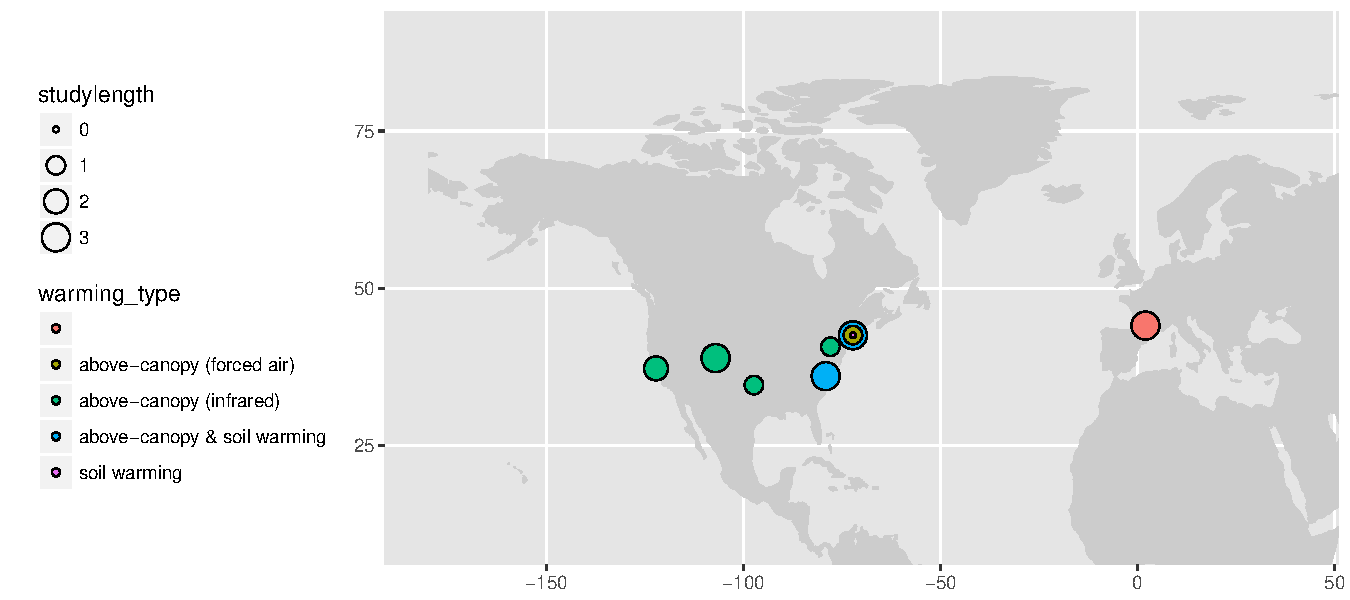
\includegraphics{maps/expsites.pdf}

Ten different phenological events were monitored across all sites:
\begin{Schunk}
\begin{Sinput}
> table(expdata$site, expdata$event)
\end{Sinput}
\begin{Soutput}
                   bbd   col  drop   ffb   ffd  ffrd   lod   lud    sd   sen
  bace             243     0     0     0     0     0   254   256     0     0
  chuine             0     0     0  3367  3284  2238     0     0     0     0
  clarkduke       8304     0     0     0     0     0 12573 13989     0     0
  clarkharvard    2527     0     0     0     0     0  4503  3698     0     0
  cleland            0     0     0     0  2368     0     0     0     0     0
  dunnermbl          0     0     0     0  9117   938     0     0     0     0
  farnsworthharv   262    45     0     0    12    20   305   170     0     0
  force              0     0     0     0   585   388  1333     0   179   551
  harvardellison    68     0   146     0     0     0   196    91     0   214
  marchin          849     0     0     0   280     0     0     0     0     0
  oklahoma           0     0     0     0   623   671     0     0     0     0
  rmbl               0     0     0     0  1071   650     0     0   476     0
\end{Soutput}
\end{Schunk}

\subsection{Phenology Data from Observational Studies}

Next, the observational data. 

\begin{Schunk}
\begin{Sinput}
> head(obsdata)
\end{Sinput}
\begin{Soutput}
    site plot event year doy       date genus   species scrub varetc cult
1 fitter <NA>   ffd 1954 130 1954-05-10  Acer campestre     0     NA   NA
2 fitter <NA>   ffd 1955 131 1955-05-11  Acer campestre     0     NA   NA
3 fitter <NA>   ffd 1956 137 1956-05-16  Acer campestre     0     NA   NA
4 fitter <NA>   ffd 1957 121 1957-05-01  Acer campestre     0     NA   NA
5 fitter <NA>   ffd 1958 128 1958-05-08  Acer campestre     0     NA   NA
6 fitter <NA>   ffd 1959 129 1959-05-09  Acer campestre     0     NA   NA
\end{Soutput}
\end{Schunk}

The observational data come from 15 sites (see "obssiteinfo.csv" file for details).

\begin{Schunk}
\begin{Sinput}
> unique(obsdata$site)
\end{Sinput}
\begin{Soutput}
 [1] fitter   harvard  hubbard  konza    niwot    mikesell concord  mohonk   marsham 
[10] fargo    washdc   bolmgren gothic   uwm      rousi   
15 Levels: bolmgren concord fargo fitter gothic harvard hubbard konza ... washdc
\end{Soutput}
\end{Schunk}
\includegraphics{Observations/Temp/map_sites.eps}

And include 7 phenological stages:
\begin{Schunk}
\begin{Sinput}
> table(obsdata$site, obsdata$event)
\end{Sinput}
\begin{Soutput}
              bbd    ffd    fld L75mdoy L95mdoy    lod    lud
  bolmgren      0   1622      0       0       0      0      0
  concord       0   9320      0       0       0      0      0
  fargo         0   4725      0       0       0      0      0
  fitter        0  13721      0       0       0      0      0
  gothic        0 162352      0       0       0      0      0
  harvard     483    284      0       0       0      0      0
  hubbard      72      0      0       0       0     72      0
  konza         0   3403      0       0       0      0      0
  marsham       0   2131    660       0       0      0      0
  mikesell    445      0      0       0       0    549    554
  mohonk        0    673      0       0       0      0      0
  niwot       648    371      0       0       0      0      0
  rousi      1021    147      0       0       0      0      0
  uwm         414      0      0     415     415      0      0
  washdc        0   7455      0       0       0      0      0
\end{Soutput}
\begin{Sinput}
> obsdata$doy <- as.numeric(obsdata$doy)
> obsagg <- aggregate(obsdata[c("doy")], obsdata[c("site", "year")], FUN=mean, na.action = na.omit)
> # simple plot, need to add a legend
> obsitez <- unique(obsdata$site)
> somecolors <- rainbow(length(obsitez))
> plot(doy~year, data=obsagg, type="n")
> for (i in seq_along(obsitez)){
+      subby <- subset(obsagg, site==obsitez[i])
+      lines(doy~year, data=subby, col=somecolors[i])
+ }
\end{Sinput}
\end{Schunk}

\subsection{Climate Data from Experiments}
We compiled daily air and soil temperature, whenever possible, as well as soil moisture or humidity data for all sites.
\begin{Schunk}
\begin{Sinput}
> head(expclim)
\end{Sinput}
\begin{Soutput}
     site temptreat preciptreat plot year doy airtemp_min airtemp_max soiltemp1_min
1 marchin         1        <NA>    1 2010   1       2.932       30.87         4.596
2 marchin         1        <NA>    1 2010  10          NA          NA            NA
3 marchin         1        <NA>    1 2010 100       6.683       32.76            NA
4 marchin         1        <NA>    1 2010 101       5.883       36.37            NA
5 marchin         1        <NA>    1 2010 102       7.922       36.90            NA
6 marchin         1        <NA>    1 2010 103       9.980       40.81            NA
  soiltemp2_min soiltemp1_max soiltemp2_max soiltemp1_mean  soilmois gdd_soil gdd_air
1            NA          8.97            NA          6.783 0.1777083   -3.217  6.9010
2            NA            NA            NA             NA        NA       NA      NA
3         12.16            NA         15.18             NA 0.1608333       NA  9.7215
4            NA            NA            NA             NA 0.1558333       NA 11.1265
5            NA            NA            NA             NA 0.1513333       NA 12.4110
6         13.58            NA         17.03             NA 0.1463333       NA 15.3950
\end{Soutput}
\end{Schunk}
The experimental climate data file has the following columns:

temptreat: temperature treatment level (1-9; these levels are defined in "expsiteinfo.csv")

preciptreat: temperature treatment level (1-2; these levels are defined in "expsiteinfo.csv")

plot

year

doy: day of year

airtemp-min: minimum daily air temperature (degrees C), measured

airtemp-max: maximum daily air temperature (degrees C), measured

soiltemp1-min: minimum daily soil temperature (degrees C), measured, depth closest to the soil surface

soiltemp2-min: minimum daily soil temperature (degrees C), measured, depth second closest to soil surface

soiltemp1-max: maximum daily soil temperature (degrees C), measured, depth closest to the soil surface

soiltemp2-max: maximum daily soil temperature (degrees C), measured, depth second closest to soil surface

soiltemp1-mean: mean daily soil temperature (degrees C), measured, depth closest to the soil surface (some studies only have data for mean, rather than min or max)

soilmos: soil moisture (percent)

\subsection{Climate Data for Observational Studies}

We extracted temperature data from Berkeley Earth Surface Temperatures (BEST) \url{http://berkeleyearth.org/}. The BEST data are daily gridded tmax and tmin, covering (for most areas) 1880-2013. We took the latitudes and longitudes for the observational phenological data sites, and found the closest BEST grid cell with at least 25 percent land area coverage (in some cases the absolute nearest grid cell was ocean, for where there are no data. Hence the land fraction threshold). The data are in comma delimited text files in Observations/Temp on github; one file for tmax and one for tmin for each site. Each row is a year and each column is a day of year (1-365 for a normal year, 1-366 for a leap year). Some sites do have missing data for some years, but most are pretty much complete.

Note: the data are too extensive to compile into a single datafile of observational climate data, so we have left them in separate files.

Here is a summary of the site info and associated BEST gridcell information (from file 
distinfo-site-BEST-.csv):


\begin{Schunk}
\begin{Soutput}
            X Lat..Site.  Lon..Site. Dist..km. Lat..BEST. Lon..BEST. Frac.Land
1      fitter   51.42000   -0.540000  9.320189       51.5       -0.5      1.00
2     concord   42.27000  -71.210000 34.959232       42.5      -71.5      1.00
3       fargo   46.51000  -96.280000 16.879558       46.5      -96.5      1.00
4    bolmgren   60.13000   16.950000 48.043302       60.5       16.5      1.00
5     harvard   42.53000  -72.190000 25.634244       42.5      -72.5      1.00
6     hubbard   43.94000  -71.750000 52.906733       43.5      -71.5      1.00
7       konza   39.13000  -96.430000 41.593559       39.5      -96.5      1.00
8      mohonk   41.77000  -74.160000 41.241097       41.5      -74.5      1.00
9       niwot   40.30000 -105.360000 25.209401       40.5     -105.5      1.00
10     gothic   38.57000 -106.590000 11.042735       38.5     -106.5      1.00
11    marsham   52.37000    1.180000 26.076351       52.5        1.5      0.59
12     washdc   38.40000  -76.700000 20.669903       38.5      -76.5      0.70
13   mikesell   41.33000  -84.090000 39.079552       41.5      -84.5      1.00
14        uwm   43.23000  -88.220000 37.610769       43.5      -88.5      1.00
15      rousi   61.80000   29.316700 34.745032       61.5       29.5      0.76
16   siernev1   36.87000   -3.690000 44.507990       36.5       -3.5      0.29
17   siernev2   37.36000   -2.560000 16.449278       37.5       -2.5      1.00
18     zacken   74.46667  -20.566667  4.205057       74.5      -20.5      0.71
19       bock   49.46344   -2.596667 79.354125       49.5       -1.5      0.44
20 augspurger   40.15000  -88.166667 48.110043       40.5      -88.5      1.00
\end{Soutput}
\end{Schunk}


The other file, map-sites.eps, plots the locations of the phenology sites (in red) and the chosen BEST gridcell (in blue):

\begin{Schunk}
\begin{Sinput}
> ## look at species numbers and overlap
> expdata$latbi <- paste(expdata$genus, expdata$species)
> obsdata$latbi <- paste(obsdata$genus, obsdata$species)
> length(unique(expdata$latbi))
\end{Sinput}
\begin{Soutput}
[1] 219
\end{Soutput}
\begin{Sinput}
> length(unique(obsdata$latbi))
\end{Sinput}
\begin{Soutput}
[1] 2143
\end{Soutput}
\begin{Sinput}
> unique(expdata$latbi)[which(unique(expdata$latbi) %in% unique(obsdata$latbi))]
\end{Sinput}
\begin{Soutput}
  [1] "Acer rubrum"                   "Carya tomentosa"              
  [3] "Quercus alba"                  "Vaccinium pallidum"           
  [5] "Vaccinium stamineum"           "Quercus rubra"                
  [7] "Chimaphila maculata"           "Hieracium venosum"            
  [9] "Thalictrum thalictroides"      "Betula lenta"                 
 [11] "Fagus grandifolia"             "Acer pensylvanicum"           
 [13] "Vaccinium corymbosum"          "Castanea dentata"             
 [15] "Prunus serotina"               "Vaccinium vacillans"          
 [17] "Viburnum acerifolium"          "Viburnum lentago"             
 [19] "Bromus hordeaceus"             "Geranium dissectum"           
 [21] "Vicia sativa"                  "Vulpia myuros"                
 [23] "Pinus taeda"                   "Nyssa sylvatica"              
 [25] "Liquidambar styraciflua"       "Pinus strobus"                
 [27] "Liriodendron tulipifera"       "Pinus virginiana"             
 [29] "Fraxinus americana"            "Quercus velutina"             
 [31] "Acer saccharum"                "Quercus phellos"              
 [33] "Cornus florida"                "Juniperus virginiana"         
 [35] "Diospyros virginiana"          "Betula alleghaniensis"        
 [37] "Carya ovata"                   "Ilex opaca"                   
 [39] "Quercus falcata"               "Quercus nigra"                
 [41] "Carya glabra"                  "Quercus stellata"             
 [43] "Quercus coccinea"              "Magnolia virginiana"          
 [45] "Cercis canadensis"             "Ulmus americana"              
 [47] "Betula papyrifera"             "Prunus pensylvanica"          
 [49] "Achillea millefolium"          "Andropogon gerardii"          
 [51] "Erigeron strigosus"            "Panicum virgatum"             
 [53] "Claytonia lanceolata"          "Campanula rotundifolia"       
 [55] "Erythronium grandiflorum"      "Eriogonum subalpinum"         
 [57] "Ipomopsis aggregata"           "Lathyrus leucanthus"          
 [59] "Amaranthus retroflexus"        "Setaria viridis"              
 [61] "Lolium perenne"                "Alliaria petiolata"           
 [63] "Allium vineale"                "Ambrosia artemisiifolia"      
 [65] "Amphicarpa bracteata"          "Arctium minus"                
 [67] "Boehmeria cylindrica"          "Carduus acanthoides"          
 [69] "Celastrus orbiculatus"         "Cirsium arvense"              
 [71] "Cirsium vulgare"               "Clematis virginiana"          
 [73] "Clinopodium vulgare"           "Conyza canadensis"            
 [75] "Cornus racemosa"               "Desmodium nudiflorum"         
 [77] "Desmodium paniculatum"         "Epilobium ciliatum"           
 [79] "Erechtites hieraciifolia"      "Erigeron philadelphicus"      
 [81] "Fragaria virginiana"           "Galium aparine"               
 [83] "Galium circaezans"             "Galium triflorum"             
 [85] "Geum canadense"                "Geranium maculatum"           
 [87] "Hackelia virginiana"           "Hamamelis virginiana"         
 [89] "Houstonia longifolia"          "Hypericum punctatum"          
 [91] "Ilex verticillata"             "Lactuca serriola"             
 [93] "Lepidium campestre"            "Lindera benzoin"              
 [95] "Lobelia inflata"               "Lysimachia quadrifolia"       
 [97] "Maianthemum canadense"         "Melampyrum lineare"           
 [99] "Mitchella repens"              "Oenothera biennis"            
[101] "Oenothera perennis"            "Ostrya virginiana"            
[103] "Oxalis stricta"                "Phytolacca americana"         
[105] "Plantago major"                "Potentilla canadensis"        
[107] "Populus grandidentata"         "Potentilla norvegica"         
[109] "Podophyllum peltatum"          "Populus tremuloides"          
[111] "Prunella vulgaris"             "Pseudognaphalium obtusifolium"
[113] "Rhus glabra"                   "Rosa multiflora"              
[115] "Rubus occidentalis"            "Sassafras albidum"            
[117] "Sambucus canadensis"           "Sisyrinchium mucronatum"      
[119] "Sonchus asper"                 "Solidago canadensis"          
[121] "Solidago juncea"               "Solidago nemoralis"           
[123] "Solidago rugosa"               "Symphyotrichum pilosum"       
[125] "Trifolium aureum"              "Trifolium pratense"           
[127] "Ulmus rubra"                   "Uvularia perfoliata"          
[129] "Veronica officinalis"          "Verbascum thapsus"            
[131] "Verbena urticifolia"           "Viola blanda"                 
[133] "Vicia cracca"                  "Viburnum prunifolium"         
[135] "Trifolium repens"              "Veronica serpyllifolia"       
[137] "Viola pubescens"               "Rumex acetosella"             
[139] "Viburnum cassinoides"          "Artemisia tridentata"         
[141] "Delphinium nuttallianum"       "Erigeron speciosus"           
[143] "Helianthella quinquenervis"    "Potentilla hippiana"          
[145] "Festuca thurberi"              "Eriogonum umbellatum"         
\end{Soutput}
\begin{Sinput}
> 
\end{Sinput}
\end{Schunk}

\end{document}
